\documentclass[12pt,letterpaper]{article}

% --- PAQUETES TIPOGRÁFICOS Y BÁSICOS ---
\usepackage[utf8]{inputenc}
\usepackage[spanish]{babel}
\usepackage{microtype}            % Mejora la justificación
\usepackage{newtxtext,newtxmath}  % Tipografía elegante compatible con pdfLaTeX
\usepackage{graphicx}
\usepackage{amsmath}
\usepackage{geometry}
\usepackage{hyperref}
\usepackage{caption}
\usepackage{enumitem}
\usepackage{fancyhdr}
\usepackage{titlesec}
\usepackage{xcolor}
\usepackage{float}     % para usar [H]
\usepackage{placeins}  % para \FloatBarrier
\usepackage{datetime2}
\usepackage{listings}
\usepackage{minted}

\setminted{
    breaklines=true,
    breakanywhere=true,
    fontsize=\small,
    frame=single,
    linenos
}

% --- GEOMETRÍA DE PÁGINA ---
\geometry{
  letterpaper,
  margin=1in,
  headheight=15pt % Corrige warning de fancyhdr
}

% --- PÁRRAFOS Y LÍNEA ---
\setlength{\parindent}{1.5em}   % Sangría inicial en párrafos
\setlength{\parskip}{0.4em}     % Pequeño espacio entre párrafos
\linespread{1.05}               % Ligeramente más aire entre líneas
\raggedbottom                   % Evita estiramientos verticales feos

% --- LISTAS COMPACTAS (sin perder legibilidad) ---
\setlist[itemize]{topsep=4pt,itemsep=2pt,parsep=2pt}
\setlist[enumerate]{topsep=4pt,itemsep=2pt,parsep=2pt}

% --- CAPTIONS ---
\captionsetup[figure]{labelfont=bf,font=small}
% \captionsetup[table]{labelfont=bf,font=small}
% \captionsetup[listing]{labelfont=bf,font=small,name=Listado}

% --- HYPERREF ---
\hypersetup{
  colorlinks=true,
  linkcolor=blue!50!black,
  urlcolor=teal!60!black,
  citecolor=purple!60!black,
  pdftitle={SimpleImgProcessing},
  pdfpagemode=UseOutlines
}

% --- ENCABEZADOS Y PIES ---
\pagestyle{fancy}
\fancyhf{}
\fancyhead[L]{SimpleImgProcessing}
\fancyhead[R]{\thepage}
\renewcommand{\headrulewidth}{0.4pt}
\renewcommand{\footrulewidth}{0pt}
\setlength{\headheight}{15pt} % Corrige el warning de fancyhdr

% --- ESTILO DE SECCIONES ---
\titleformat{\section}{\large\bfseries}{\thesection}{0.6em}{}
\titleformat{\subsection}{\normalsize\bfseries}{\thesubsection}{0.6em}{}
\titleformat{\subsubsection}{\normalsize\itshape}{\thesubsubsection}{0.6em}{}
\titlespacing*{\section}{0pt}{0.8em}{0.4em}
\titlespacing*{\subsection}{0pt}{0.6em}{0.3em}
\titlespacing*{\subsubsection}{0pt}{0.5em}{0.25em}

% --- RUTA DE IMÁGENES (opcional) ---
% \graphicspath{{figuras/}}

% --- MODO DRAFT PARA COMPILACIÓN RÁPIDA ---
% Si tienes problemas de timeout, descomenta la siguiente línea:
% \usepackage[draft]{graphicx}  % Esto evita cargar las imágenes completas

% ==============================
% INICIO DEL DOCUMENTO
% ==============================
\begin{document}

% ========== CARÁTULA ==========
\begin{titlepage}
  \centering
  \vspace*{0.5cm}
  \includegraphics[width=0.5\textwidth]{logo.jpg}\par
  \vspace{1.2cm}

  {\Large\scshape Instituto Tecnológico y de Estudios Superiores de Monterrey\par}
  \vspace{2.2cm}

  {\huge\bfseries Actividad 2.2 Google Colab\par
   \vspace{0.2cm}
   \emph{SimpleImgProcessing}\par}
  \vspace{2.2cm}

  {\Large\bfseries Equipo 5\par}
  {\normalsize\bfseries A01796323 Benjamín Cisneros Barraza\par}
  {\normalsize\bfseries A01066264 Carlos Pano Hernandez\par}
  {\normalsize\bfseries A01795590 Edgar Omar Cruz Mendoza\par}
  {\normalsize\bfseries A01275322 Jonatan Israel Meza Mendoza\par}
  
  \vspace{1.2cm}

  \begin{flushleft}
    \normalsize \textbf{Profesor Titular:} Dr. Gilberto Ochoa Ruiz\\
    \normalsize \textbf{Profesor Asistente:} MIP Ma. del Refugio Meléndez Alfaro\\
    \normalsize \textbf{Profesor Asistente:} Iván Reyes Amezcua
  \end{flushleft}

  \vfill

  \begin{flushright}
    \normalsize Visión computacional para imágenes y video\\
    \normalsize 21 de Septiembre de 2025
  \end{flushright}
\end{titlepage}

\setcounter{page}{1} % Reinicia numeración tras la carátula

% ========== RESUMEN ==========
\section*{Resumen}

<<Resumen del trabajo>>
% ========== OBJETIVOS ==========
\section*{Objetivos del <<TipoDocumento>>}

\begin{enumerate}
  \item <<Objetivo1>>
  \item <<Objetivo2>>
  \item <<Objetivo3>>
\end{enumerate}

\newpage

% ========== TABLA DE CONTENIDOS ==========
\tableofcontents
\newpage

% ========== TABLA DE FIGURAS ==========
\listoffigures
\newpage

% ========== INTRODUCCIÓN ==========
\section{Introducción}

En el campo de la visión por computadora y el procesamiento de imágenes, las transformaciones a nivel de píxel son técnicas fundamentales. Estas transformaciones se utilizan para modificar la intensidad, el \textbf{color o el contraste de una imagen}, lo cual es crucial para tareas como la aumentación de datos en aprendizaje automático, la mejora de imágenes para aplicaciones específicas (p. ej., imágenes médicas, astronomía) y la extracción de características para el análisis. Este proyecto explora varias transformaciones clave a nivel de píxel, incluyendo ajustes fotométricos, la inversión negativa, la corrección de gamma y la sustracción de imágenes.


\newpage

\section{Desarrollo de actividades}

<<Texto>>

\subsection{Carga de imágenes}
Para desarrollar esta primera actividad, se realizó la carga de 3 imágenes de nuestro carrete. El código se muestra a continuación. 

\begin{minted}{python}
fig, axes = plt.subplots(1, 3, figsize=(15, 5))

axes[0].imshow(img1)
axes[0].set_title('Image 1')
axes[0].axis('off')

axes[1].imshow(img2)
axes[1].set_title('Image 2')
axes[1].axis('off')

axes[2].imshow(img3)
axes[2].set_title('Image 3')
axes[2].axis('off')

plt.tight_layout()
plt.show()
\end{minted}

\begin{figure}[H]
  \centering
  \includegraphics[width=0.8\linewidth]{figuras/carga_imagenes.png}
  \caption{Carga y visualización de imágenes}
  \label{fig:carga_imagenes}
\end{figure}

Referencia a imagen \ref{fig:carga_imagenes}


\subsection{Transformaciones Pixel a Pixel}

Para esta actividad, investigamos tres tipos de transformaciones:


\subsubsection{Transformación logarítmica}

Esta transformación expande el rango de intensidad de los píxeles oscuros mientras comprime el de los brillantes. Es útil para imágenes con un rango estrecho de valores oscuros, ya que ayuda a revelar detalles en las áreas de sombra.


Código:

\begin{minted}{python}
# Ensure img1 is uint8 RGB for OpenCV ops
if img1.dtype != np.uint8:
    img1_u8 = (cv2.normalize(img1, None, 0, 255, cv2.NORM_MINMAX)).astype(np.uint8)
else:
    img1_u8 = img1

# Convert to grayscale for histogram-based ops
img1_gray = cv2.cvtColor(img1_u8, cv2.COLOR_RGB2GRAY)

# 1) Logarithmic transform (on grayscale)
c_log = 255.0 / np.log1p(255.0)
img_log = (c_log * np.log1p(img1_gray.astype(np.float32))).clip(0, 255).astype(np.uint8)
\end{minted}

Resultados:
\begin{figure}[H]
  \centering
  \includegraphics[width=0.8\linewidth]{figuras/transformacion_log.png}
  \caption{Transformación Logarítmica: Comparación de imágenes}
  \label{fig:transformacion_log}
\end{figure}

Referencia a imagen \ref{fig:transformacion_log}

Discusión Justificación:

La transformación logarítmica expande el rango de intensidad de los píxeles oscuros y comprime el de los brillantes. La imagen de ejemplo (el perrito de una amiga: 'Cookie' y 'Copito') es convertida a escala de grises y luego se le aplica esta transformación. El resultado es una imagen notablemente más clara donde se revelan detalles en las áreas de sombra, demostrando la efectividad de esta técnica para imágenes con un rango estrecho de valores oscuros.


\subsubsection{Estiramiento de contraste}
Esta técnica mejora el contraste general mapeando linealmente el rango de intensidad de píxeles original a un nuevo rango más amplio (p. ej., de 0 a 255). Es efectiva cuando los valores de píxel de una imagen se agrupan en un rango pequeño, resultando en una apariencia de bajo contraste.


Código:
\begin{minted}{python}
# 2) Contrast stretching using percentiles to avoid outliers
p_low, p_high = np.percentile(img1_gray, (2, 98))
if p_high <= p_low:
    p_low, p_high = img1_gray.min(), img1_gray.max()
img_cs = np.clip((img1_gray - p_low) * (255.0 / max(1.0, (p_high - p_low))), 0, 255).astype(np.uint8)
\end{minted}

Resultados:

\begin{figure}[H]
  \centering
  \includegraphics[width=0.8\linewidth]{figuras/estiramiento_de_contraste.png}
  \caption{Estiramiento de Contraste}
  \label{fig:estiramiento_de_contraste}
\end{figure}

Referencia a imagen \ref{fig:estiramiento_de_contraste}

Discusión/Justificación:

\begin{figure}[H]
  \centering
  \includegraphics[width=0.8\linewidth]{figuras/estiramiento_de_contraste_justificacion.png}
  \caption{Comparativa de Histogramas de escalas de grises entre Original y Estiramiento de contraste}
  \label{fig:estiramiento_de_contraste_justificacion}
\end{figure}

En la figura \ref{fig:estiramiento_de_contraste_justificacion} se muestra que el estiramiento de contraste tiene una mejora general, pero la de la ecualización del histograma parece tener un contraste aún más equilibrado y uniforme.

\subsubsection{Ecualización del histograma}
Este método redistribuye los valores de intensidad para aplanar el histograma de la imagen, lo que mejora el contraste en toda la imagen. Es particularmente eficaz para imágenes con muy bajo contraste y puede revelar detalles que de otra manera no serían visibles.


Código:
\begin{minted}{python}
# 3) Histogram equalization
img_eq = cv2.equalizeHist(img1_gray)
\end{minted}

Resultados:
<<Colocar resultados>>


Discusión/Justificación:

<<Colocar imagen>>
La comparación de los histogramas confirma la diferencia. El histograma original muestra una concentración de valores en un rango pequeño. El histograma con estiramiento de contraste muestra los valores más dispersos. El histograma de la ecualización muestra una distribución más uniforme en todo el rango de 0 a 255, lo que justifica la mejora visual en el contraste.

Histogramas:

<<Colocar imagen>>

\subsubsection{Negativo de Imagen}

La inversión de una imagen, o la obtención de su negativo, es una transformación a nivel de píxel donde la intensidad de cada píxel se resta del valor de intensidad máximo posible. Esta técnica es de gran valor en el análisis de películas de radiología, ya que puede hacer que los detalles de bajo contraste sean más visibles.

En las películas de rayos X tradicionales, los huesos y tejidos densos aparecen como áreas claras sobre un fondo oscuro. Para este ejercicio, el uso de esta técnica para la detección de billetes falsos resulta altamente conveniente, pues resalta detalles difíciles de detectar a simple vista.



Código:
\begin{minted}{python}
plt.tight_layout()
plt.show()
# Grayscale histogram for each bill and its negative
def plot_gray_hist(ax, image, title):
    gray = cv2.cvtColor(image, cv2.COLOR_RGB2GRAY)
    ax.hist(gray.ravel(), bins=256, range=(0,256), color='black')
    ax.set_title(title)
    ax.set_xlim(0,256)

fig, axes = plt.subplots(2, 2, figsize=(12, 8))

plot_gray_hist(axes[0, 0], bill1, 'Bill 1 - Histogram (Original)')
plot_gray_hist(axes[0, 1], neg_bill1, 'Bill 1 - Histogram (Negative)')
plot_gray_hist(axes[1, 0], bill2, 'Bill 2 - Histogram (Original)')
plot_gray_hist(axes[1, 1], neg_bill2, 'Bill 2 - Histogram (Negative)')

plt.tight_layout()
plt.show()
\end{minted}

Resultados:
<<Colocar resultados>>


Discusión/Justificación:

Análisis Visual: Al invertir la imagen, los detalles de los billetes que son difíciles de ver a simple vista se vuelven más evidentes. Las marcas de seguridad o texturas que eran claras se vuelven oscuras y viceversa.

Análisis del Histograma: Los histogramas de los billetes originales y sus negativos son inversos. Los picos de intensidad que estaban en el lado derecho (brillante) del histograma original se mueven al lado izquierdo (oscuro) en el histograma negativo, y viceversa. Esto refleja el cambio de luminancia en la imagen.

\subsubsection{Corrección de Gamma}

La corrección de gamma es una operación no lineal utilizada para codificar o decodificar la luminancia en las imágenes. Es especialmente útil en campos como la astronomía, donde ayuda a equilibrar la representación visual de objetos celestes muy brillantes y muy oscuros.
En las imágenes astronómicas, los objetos tenues como las nebulosas y las galaxias distantes tienen valores de píxel muy bajos en comparación con las estrellas brillantes. Un valor de gamma menor que 1 ($\gamma < 1$) ilumina los tonos medios y las sombras, haciendo que los detalles tenues sean más visibles sin saturar las estrellas brillantes. Por el contrario, un valor de gamma mayor que 1 ($\gamma > 1$) oscurece la imagen, lo que puede usarse para reducir el ruido de fondo.

El siguiente código crea una función que aplica la Corrección Gamma:

\begin{minted}{python}
def apply_gamma(image_gray, gamma):
    invGamma = 1.0 / gamma
    table = np.array([((i / 255.0) ** invGamma) * 255 for i in np.arange(256)]).astype("uint8")
    return cv2.LUT(image_gray, table)

# List of gammas to test (adjust as needed)
gammas = [0.3, 0.5, 0.7, 0.9, 1.0, 1.2, 1.5, 2.0]
results = [(g, apply_gamma(imgPopo, g)) for g in gammas]

# Show original + corrections in a 3x3 grid
fig, axes = plt.subplots(3, 3, figsize=(12, 12))
axes = axes.ravel()

# Position 0: Original
axes[0].imshow(imgPopo, cmap='gray')
axes[0].set_title('Original')
axes[0].axis('off')

# Rest: different gammas
for ax, (g, img_c) in zip(axes[1:], results):
    ax.imshow(img_c, cmap='gray')
    ax.set_title(f'gamma={g}')
    ax.axis('off')

# Hide extra axes if any
for k in range(1 + len(results), len(axes)):
    axes[k].axis('off')

plt.tight_layout()
plt.show()
\end{minted}


\begin{figure}[H]
  \centering
  \includegraphics[width=0.5\linewidth]{figuras/correccion_gamma.png}
  \caption{Corrección Gamma: Múltiples transformaciones}
  \label{fig:correccion_gamma}
\end{figure}

La Figura \ref{fig:correccion_gamma} muestra diferentes imágenes producidas variando los valores de $\gamma$, donde se puede observar lo siguiente:

\begin{itemize}
  \item \textbf{$\gamma < 1$}: La imagen se vuelve progresivamente más brillante. Los tonos medios y las sombras se iluminan, haciendo que los detalles tenues sean más visibles sin saturar las partes brillantes.
  \item \textbf{$\gamma > 1$}: La imagen se oscurece. Los tonos medios se vuelven más oscuros, lo que puede ser útil para reducir el ruido de fondo.
  \item \textbf{$\gamma = 1$}: La imagen permanece sin cambios, sirviendo como el punto de referencia.
\end{itemize}

\subsubsection{Sustracción de Imágenes}

La sustracción de imágenes es una técnica para detectar cambios entre dos imágenes capturadas en momentos diferentes pero desde el mismo punto de vista. Se aplica ampliamente en la vigilancia de seguridad para detectar movimiento o la aparición de nuevos objetos en una escena.

Al restar una imagen de fondo de referencia de un nuevo fotograma, cualquier valor de píxel que no sea cero representa un cambio. Este método crea una máscara  de cambio que aísla los objetos en movimiento del fondo estático. Después de un simple umbral y operaciones morfológicas para limpiar el ruido, la máscara de cambio se puede usar para identificar y localizar intrusos u otros eventos significativos, convirtiéndose en un método potente y de bajo costo para sistemas de monitoreo en tiempo real.

En nuestro ejemplo, las figuras \ref{fig:sustraccion_referencia} y \ref{fig:sustraccion_actual} representan la imagen de referencia e imagen actual respectivamente.

\begin{figure}[H]
  \centering
  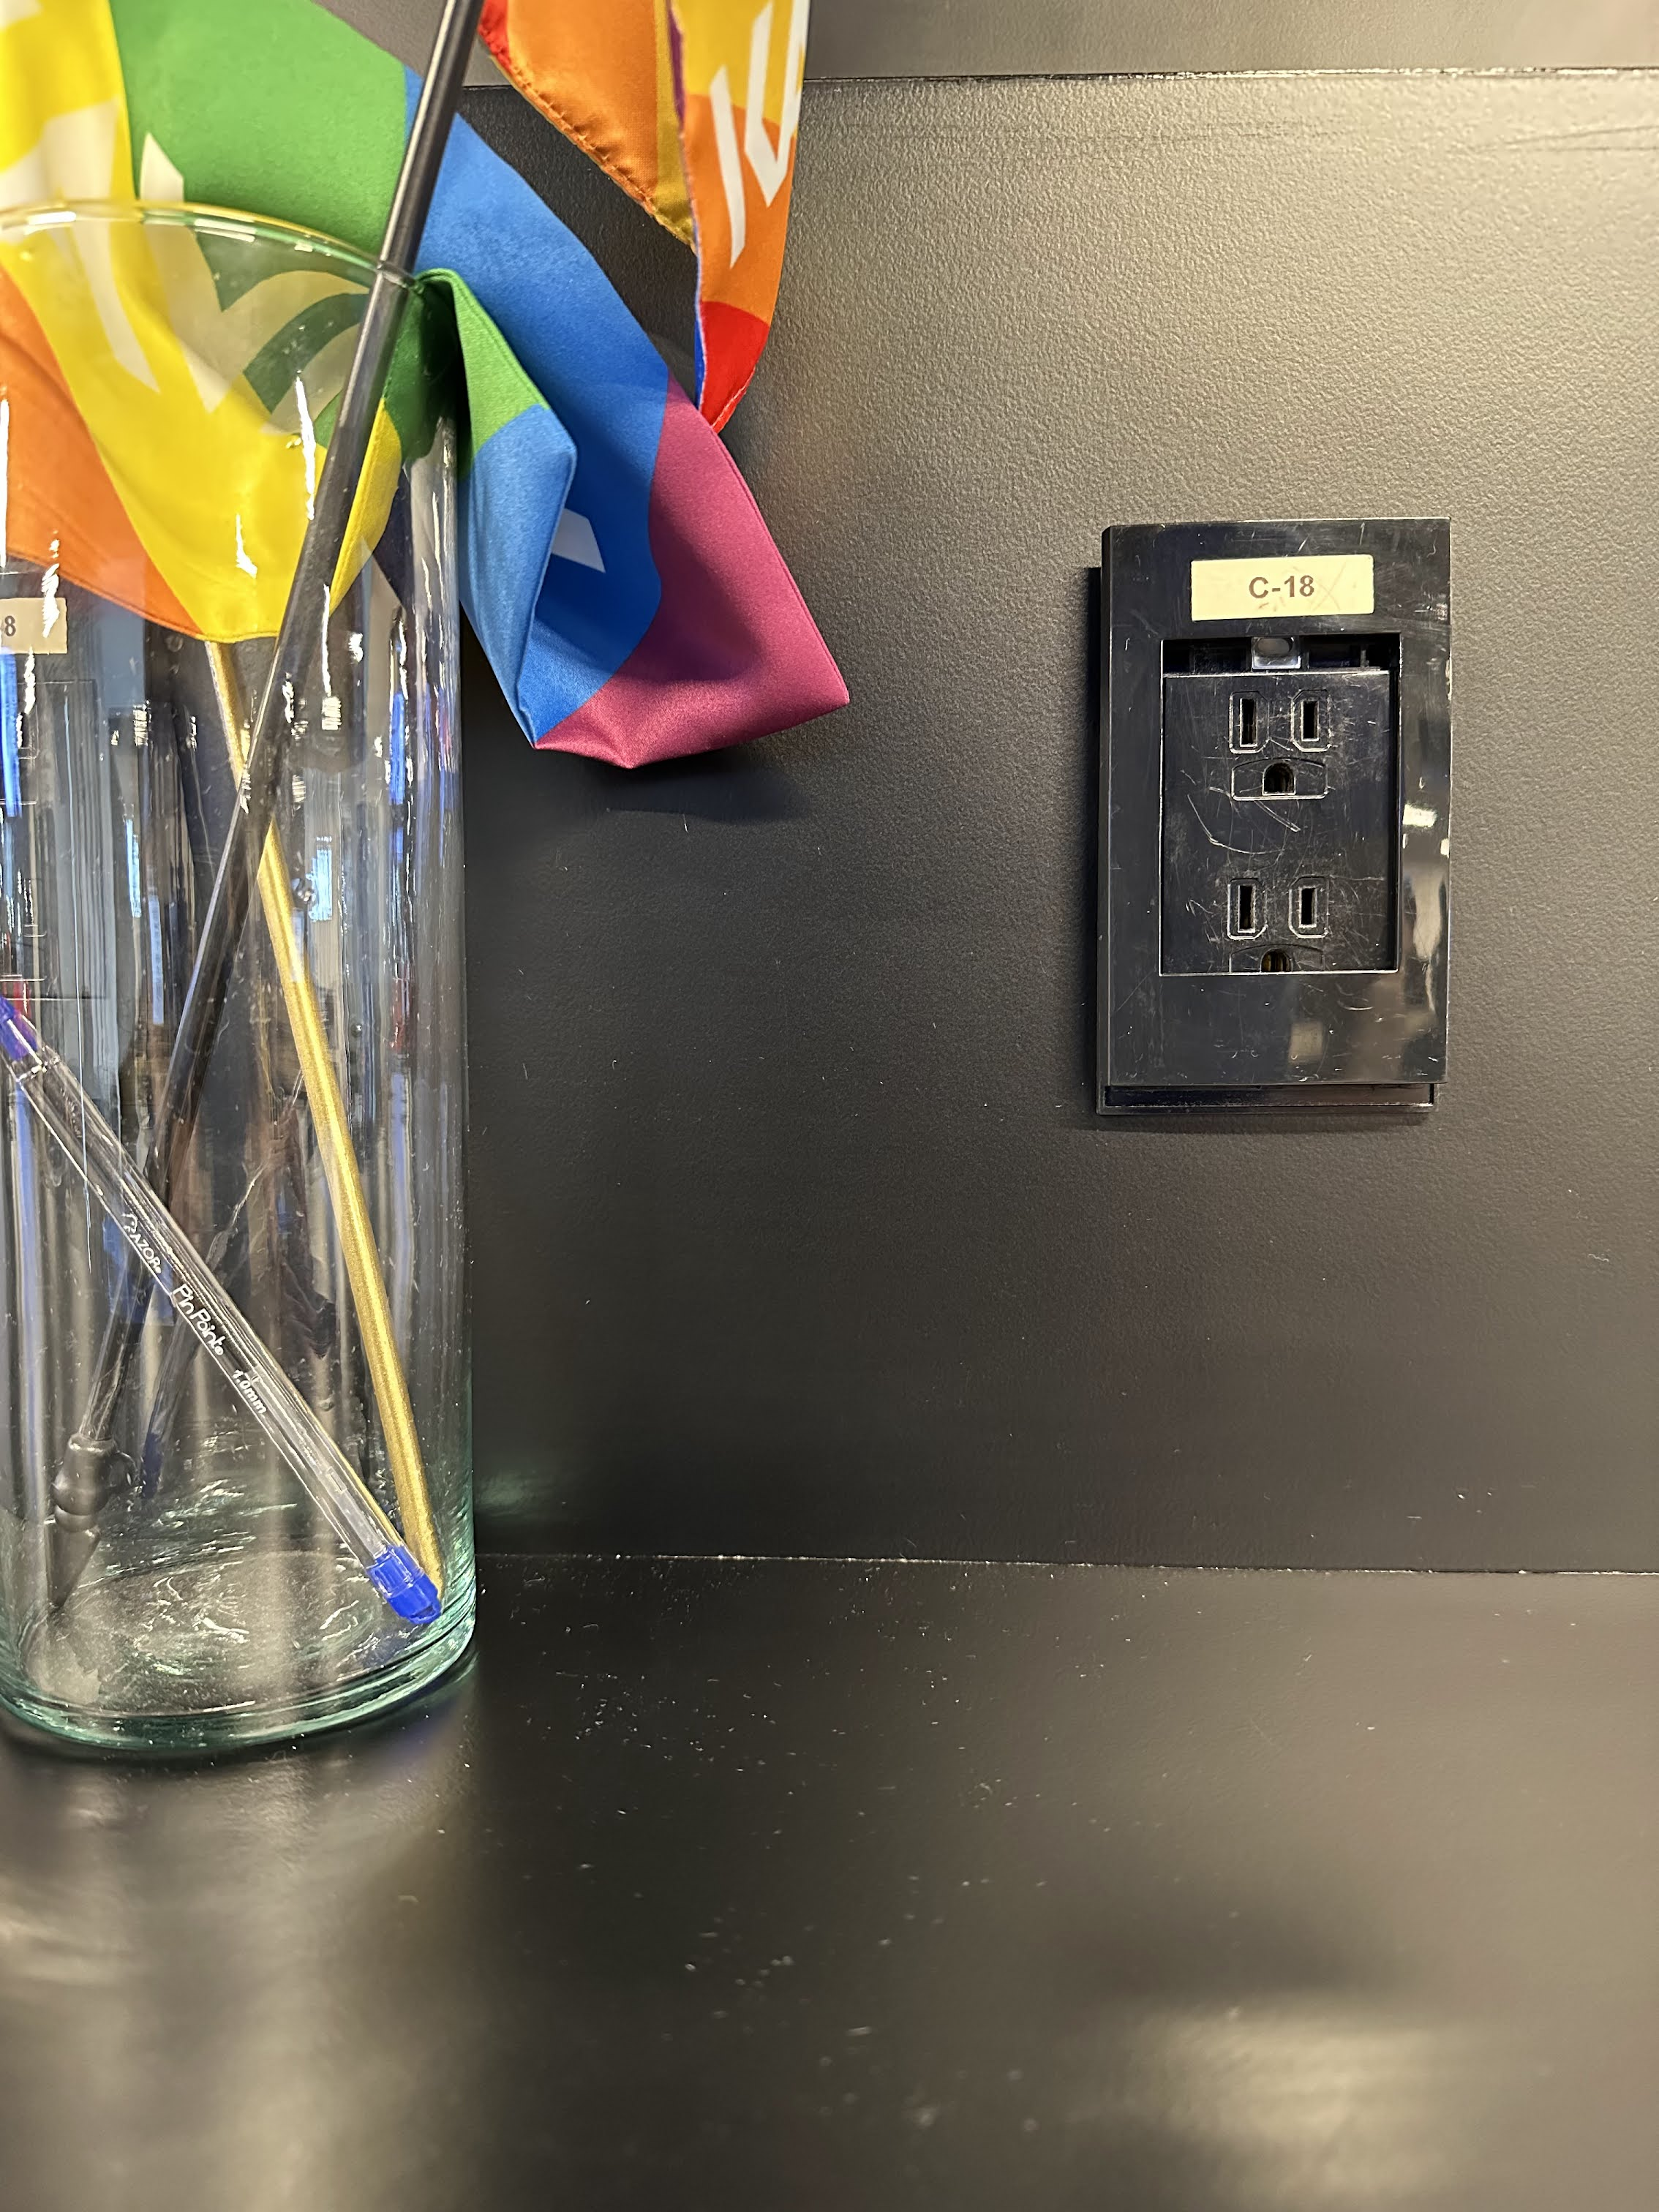
\includegraphics[width=0.5\linewidth]{../data/data-substraction-sample/img-1.jpg}
  \caption{Sustracción de Imágenes: Imagen de Referencia}
  \label{fig:sustraccion_referencia}
\end{figure}

\begin{figure}[H]
  \centering
  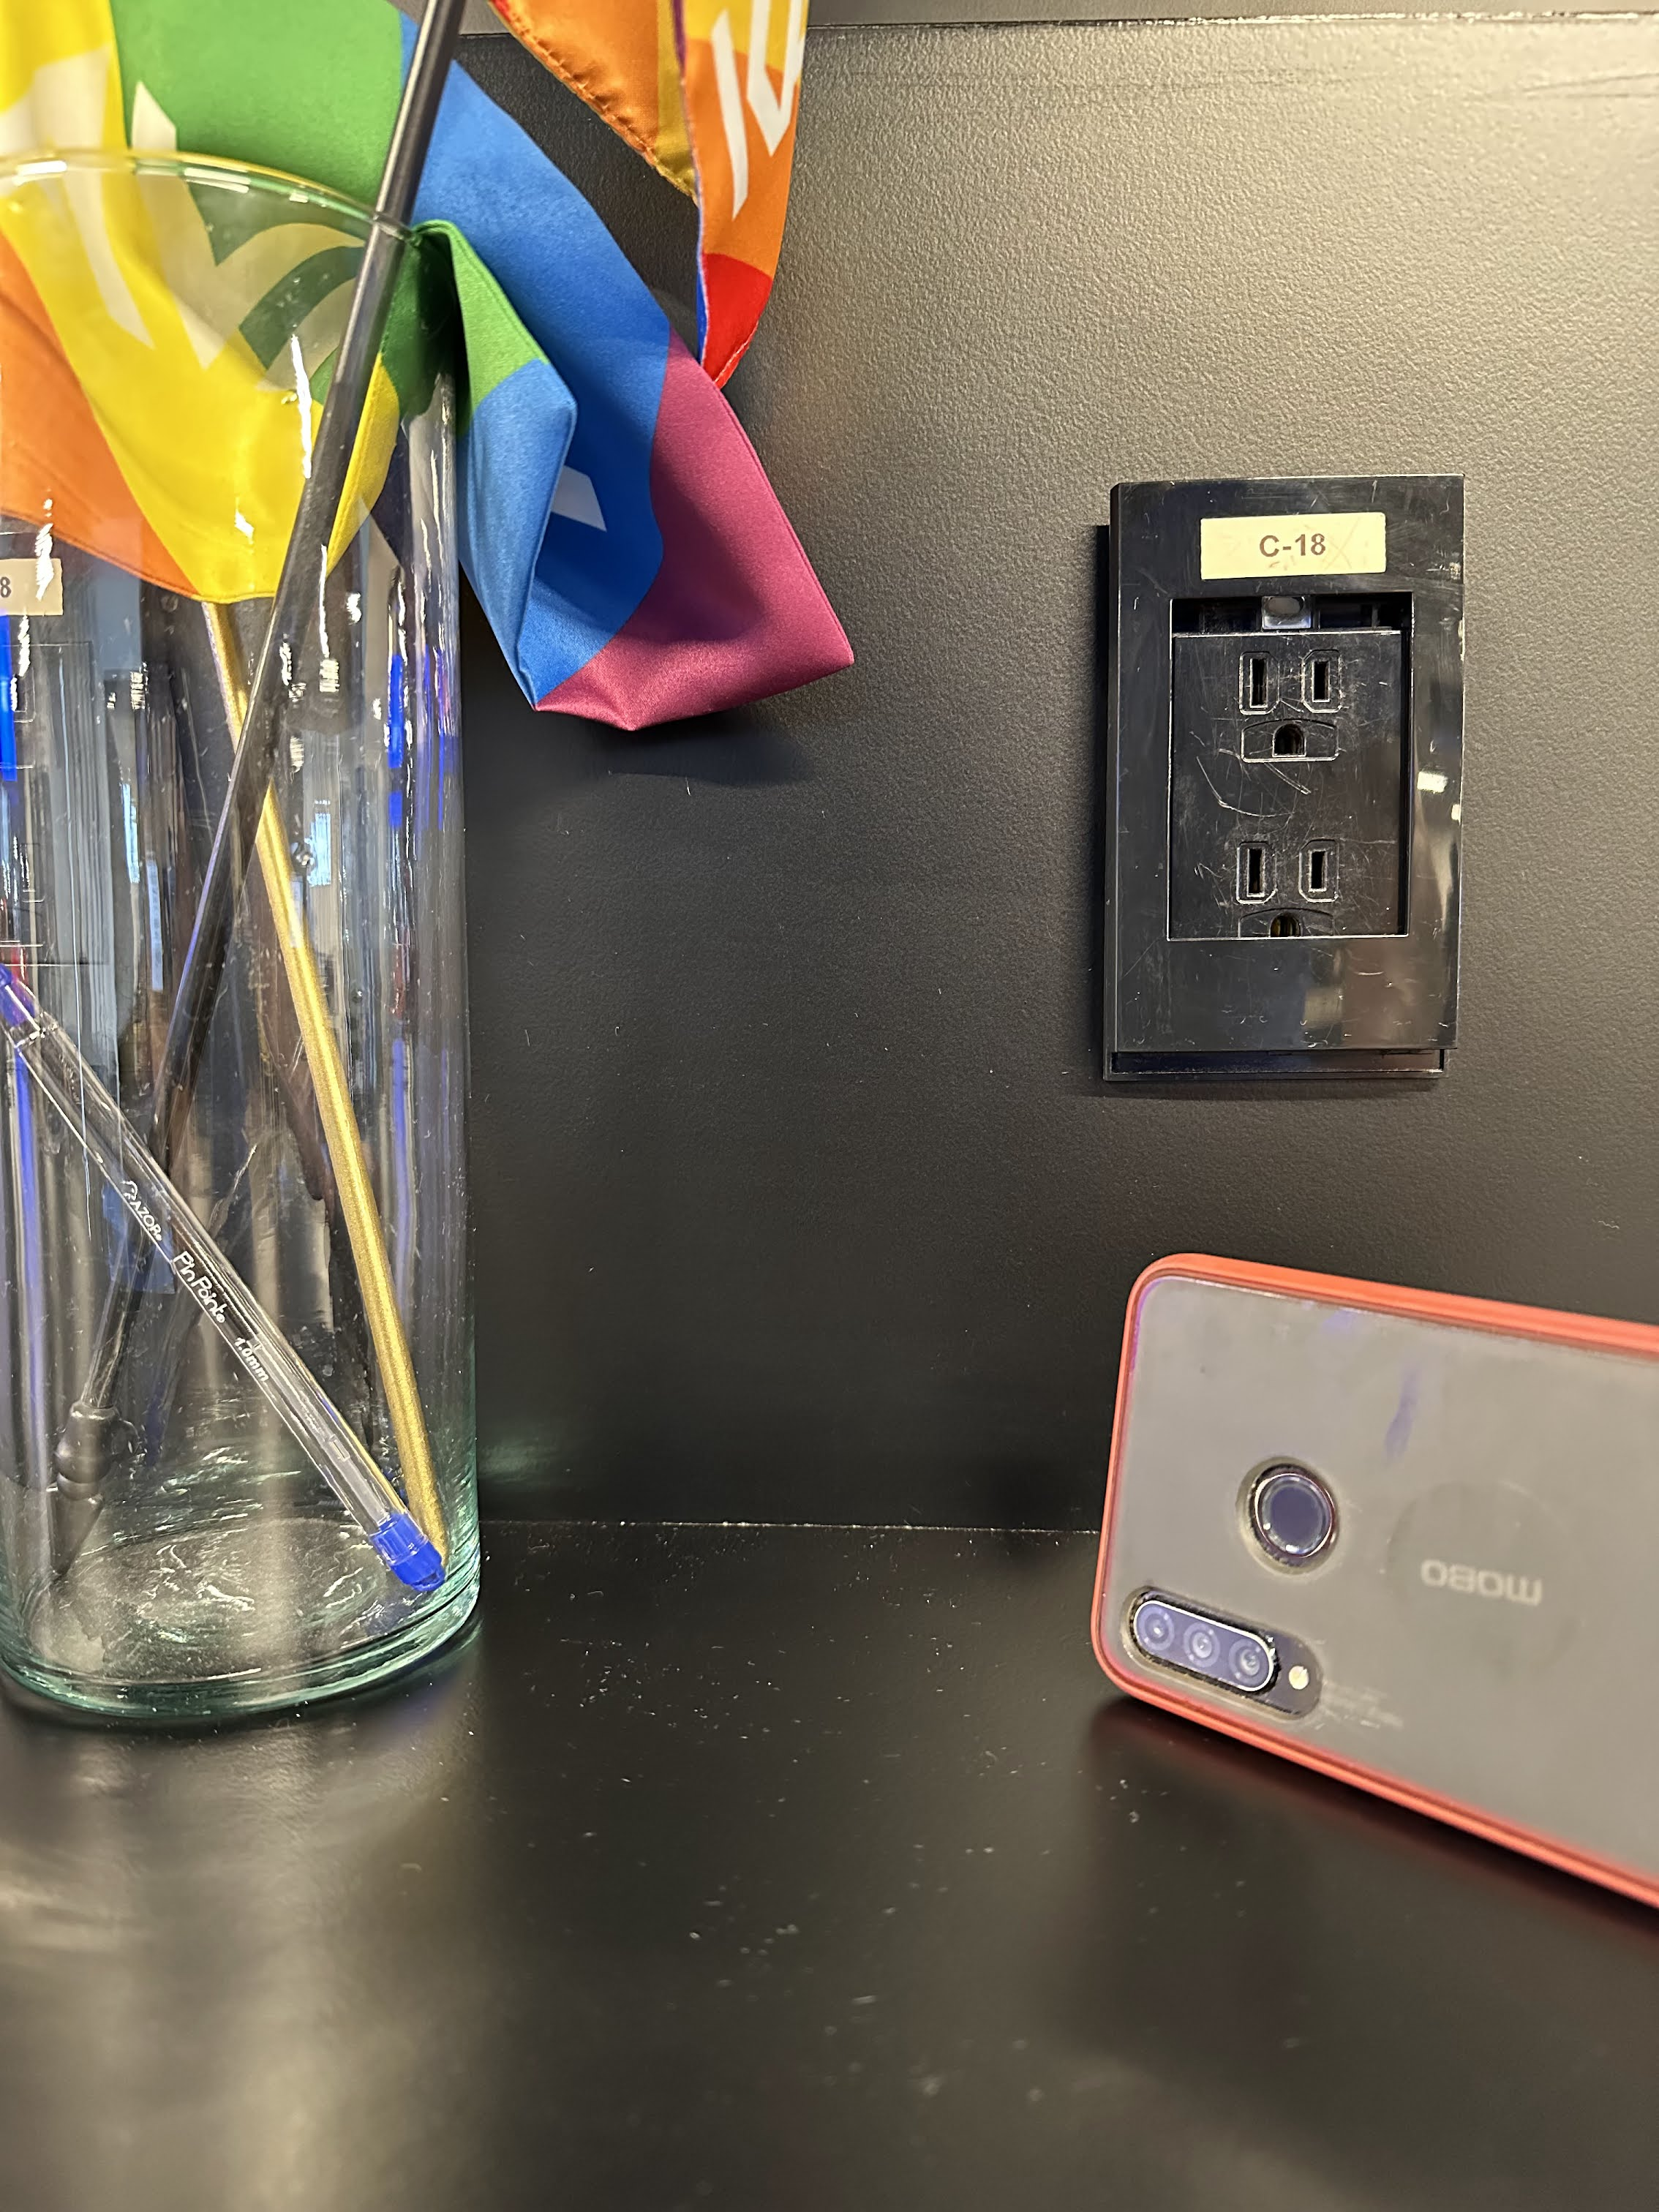
\includegraphics[width=0.5\linewidth]{../data/data-substraction-sample/img-2.jpg}
  \caption{Sustracción de Imágenes: Imagen actual}
  \label{fig:sustraccion_actual}
\end{figure}

El siguiente código nos permite realizar la sustracción de imágenes y detectar los objetos nuevos:


\begin{minted}{python}
imgV1 = mpimg.imread('data/data-substraction-sample/img-1.jpg')
imgV2 = mpimg.imread('data/data-substraction-sample/img-2.jpg')

# Ensure both images have the same shape for subtraction
if imgV1.shape != imgV2.shape:
    # Resize the second image to match the first
    imgV2_resized = cv2.resize(imgV2, (imgV1.shape[1], imgV1.shape[0]))
else:
    imgV2_resized = imgV2

# Convert to grayscale for better processing
if imgV1.ndim == 3:
    gray1 = cv2.cvtColor(imgV1, cv2.COLOR_RGB2GRAY)
else:
    gray1 = imgV1

if imgV2_resized.ndim == 3:
    gray2 = cv2.cvtColor(imgV2_resized, cv2.COLOR_RGB2GRAY)
else:
    gray2 = imgV2_resized

# Ensure 8-bit
if gray1.dtype != np.uint8:
    gray1 = cv2.normalize(gray1, None, 0, 255, cv2.NORM_MINMAX).astype(np.uint8)
if gray2.dtype != np.uint8:
    gray2 = cv2.normalize(gray2, None, 0, 255, cv2.NORM_MINMAX).astype(np.uint8)

# Detect NEW objects: objects that appear in img2 but not in img1
# Method: Find regions where img2 is significantly brighter than img1
diff_new = cv2.subtract(gray2, gray1)  # Only positive differences (new objects)

# Apply threshold to isolate new objects
_, mask_new = cv2.threshold(diff_new, 30, 255, cv2.THRESH_BINARY)  # Adjust threshold as needed

# Morphological operations to clean up the mask
kernel = np.ones((5, 5), np.uint8)
mask_clean = cv2.morphologyEx(mask_new, cv2.MORPH_OPEN, kernel, iterations=2)
mask_clean = cv2.morphologyEx(mask_clean, cv2.MORPH_CLOSE, kernel, iterations=3)

# Find contours of new objects
contours, _ = cv2.findContours(mask_clean, cv2.RETR_EXTERNAL, cv2.CHAIN_APPROX_SIMPLE)

# Filter and draw bounding boxes for new objects
vis = imgV2_resized.copy()
if vis.ndim == 2:
    vis = cv2.cvtColor(vis, cv2.COLOR_GRAY2RGB)

new_objects = []
for c in contours:
    x, y, w, h = cv2.boundingRect(c)
    area = w * h
    if area < 100:  # Filter out very small objects
        continue
    new_objects.append((x, y, w, h))
    cv2.rectangle(vis, (x, y), (x + w, y + h), (0, 255, 0), 2)  # Green for new objects
    cv2.putText(vis, f'New {len(new_objects)}', (x, y-10), cv2.FONT_HERSHEY_SIMPLEX, 0.7, (0, 255, 0), 2)

# Summary metrics for new objects only
num_new_objects = len(new_objects)
areas = [w * h for (_, _, w, h) in new_objects]
area_min = min(areas) if areas else 0
area_max = max(areas) if areas else 0

# Visualization
fig, axes = plt.subplots(1, 4, figsize=(20, 5))
axes[0].imshow(imgV1)
axes[0].set_title('Image 1 (Reference)')
axes[0].axis('off')

axes[1].imshow(imgV2_resized)
axes[1].set_title('Image 2 (Current)')
axes[1].axis('off')

axes[2].imshow(mask_clean, cmap='gray')
axes[2].set_title('New Objects Mask')
axes[2].axis('off')

axes[3].imshow(vis)
axes[3].set_title(f'NEW Objects Detected: {num_new_objects}\nArea range: {area_min}-{area_max}')
axes[3].axis('off')

plt.tight_layout()
plt.show()

print(f"Detection Summary:")
print(f"- Total new objects found: {num_new_objects}")
print(f"- Area range: {area_min} - {area_max} pixels")
if new_objects:
    print(f"- Object locations: {new_objects}")
else:
    print("- No new objects detected")
\end{minted}


\begin{figure}[H]
  \centering
  \includegraphics[width=0.5\linewidth]{figuras/sustraccion_mascara.png}
  \caption{Sustracción de Imágenes: Máscara de nuevos objetos}
  \label{fig:sustraccion_mascara}
\end{figure}

\begin{figure}[H]
  \centering
  \includegraphics[width=0.5\linewidth]{figuras/sustraccion_objetos.png}
  \caption{Sustracción de Imágenes: Objetos detectados}
  \label{fig:sustraccion_objetos}
\end{figure}

Se observa que como resultado de la sustracción se produce una máscara de objetos nuevos (Figura \ref{fig:sustraccion_mascara}) que es predominantemente negra. Las áreas que han cambiado (donde está la caja de los audífonos) se muestran en blanco, creando un mapa que aísla el objeto en movimiento del fondo estático. La imagen final (figura \ref{fig:sustraccion_objetos}) superpone esta detección, mostrando el audífono enmarcado y los detalles de los objetos detectados. Este proceso es efectivo y de bajo costo para sistemas de monitoreo en tiempo real.

\newpage

\section{Conclusiones}

El proyecto exploró y demostró con éxito varias transformaciones fundamentales a nivel de píxel en el procesamiento de imágenes, cada una con una aplicación única. La transformación logarítmica, el estiramiento de contraste y la ecualización del histograma demostraron ser herramientas efectivas para la aumentación de datos y la mejora fotométrica, revelando detalles que no eran evidentes en las imágenes originales. 

\newpage

% ==============================
% REFERENCIAS - SOLO UNA VEZ
% ==============================
\begin{thebibliography}{99}

\bibitem{anitha2018}
P. S. Anitha, P. Lakshmi Priya. (2018). A Survey on Image Enhancement Techniques. International Journal of Scientific Research in Computer Science and Engineering.

\bibitem{gonzalez2018}
Rafael C. Gonzalez, Richard E. Woods. (2018). Digital Image Processing. 4th Edition. Pearson.

\bibitem{opencpythontutorials2023}
OpenCV-Python Tutorials. (2023). OpenCV Official Documentation. Available at: https://docs.opencv.org/4.x/

%% Debemos usar Wikipedia como referencia?
\bibitem{wikipedia2023}
Wikipedia. (2023). Gamma correction. Available at: \url{https://en.wikipedia.org/wiki/Gamma_correction}
%% Estos son ejemplos
\bibitem{aguilar2020}
Aguilar-Alvarado, J. V., \& Campoverde-Molina, M. A. (2020). Clasificación de frutas basadas en redes neuronales convolucionales. \textit{Polo del Conocimiento, 5(1)}, 3–22. \url{https://dialnet.unirioja.es/descarga/articulo/7436055.pdf}

\bibitem{calonder2010}
Calonder, M., Lepetit, V., Strecha, C., \& Fua, P. (2010). BRIEF: Binary robust independent elementary features. \textit{European Conference on Computer Vision}, 778--792.

\bibitem{chen2018}
Chen, L. C., Zhu, Y., Papandreou, G., Schroff, F., \& Adam, H. (2018). Encoder-decoder with atrous separable convolution for semantic image segmentation. \textit{Proceedings of the European Conference on Computer Vision (ECCV)}, 801--818.

\bibitem{gonzalez2018}
Gonzalez, R. C., \& Woods, R. E. (2018). \textit{Digital image processing} (4th ed.). Pearson.

\bibitem{gruponortenita2025}
Grupo La Norteñita. (s.f.). \textit{Empaque}. \url{https://www.grupolanortenita.com/empaque}

\bibitem{he2017}
He, K., Gkioxari, G., Dollár, P., \& Girshick, R. (2017). Mask R-CNN. \textit{Proceedings of the IEEE International Conference on Computer Vision}, 2961--2969.

\bibitem{lowe2004}
Lowe, D. G. (2004). Distinctive image features from scale-invariant keypoints. \textit{International Journal of Computer Vision}, 60(2), 91--110.

\bibitem{mafroda}
MAF RODA. (s.f.). \textit{Su tecnología Globalscan 7 gana en fiabilidad, sencillez y precisión}. Revista Mercados. \url{https://www.3-22.eu/maf-roda-peaches-globalscan-7/}

\bibitem{montoya2014}
Montoya Holguín, C., Cortés Osorio, J. A., \& Chaves Osorio, J. A. (2014). Sistema automático de reconocimiento de frutas basado en visión por computador. Ingeniare. \textit{Revista Chilena de Ingeniería, 22(4)}, 504–516. \url{https://doi.org/10.4067/S0718-33052014000400006}

\bibitem{ochoa2023a}
Ochoa, G. (2023a). \textit{Bienvenida al curso} [Video]. Instituto Tecnológico y de Estudios Superiores de Monterrey. Visión computacional para imágenes y video.

\bibitem{ochoa2023b}
Ochoa, G. (2023b). \textit{Módulo 1. Introducción y objetivos} [Video]. Instituto Tecnológico y de Estudios Superiores de Monterrey. Visión computacional para imágenes y video.

\bibitem{ochoa2023c}
Ochoa, G. (2023c). \textit{PPT: Visión computacional para imágenes y video - Módulo 1, Tema 1.1 Introducción} [Presentación de PowerPoint]. Instituto Tecnológico y de Estudios Superiores de Monterrey.

\bibitem{rosten2006}
Rosten, E., \& Drummond, T. (2006). Machine learning for high-speed corner detection. \textit{European Conference on Computer Vision}, 430--443.

\bibitem{rublee2011}
Rublee, E., Rabaud, V., Konolige, K., \& Bradski, G. (2011). ORB: An efficient alternative to SIFT or SURF. \textit{2011 International Conference on Computer Vision}, 2564--2571.

\bibitem{szeliski2022}
Szeliski, R. (2022). \textit{Computer vision: Algorithms and applications} (2nd ed.). Springer.


\end{thebibliography}

% ==============================
% NOTAS PARA RESOLVER PROBLEMAS DE COMPILACIÓN
% ==============================
% Si experimentas timeout en la compilación:
% 
% 1. IMÁGENES: Optimiza las imágenes antes de subirlas
%    - Reduce la resolución a 150-300 DPI máximo
%    - Usa formatos comprimidos: JPG para fotos (calidad 80-90%)
%    - Redimensiona a tamaño real de uso (no más de 1500px de ancho)
%    - Herramientas: ImageMagick, TinyPNG, o Squoosh.app
%
% 2. COMPILACIÓN RÁPIDA: Para pruebas, usa modo draft
%    - Cambia \usepackage{graphicx} por \usepackage[draft]{graphicx}
%    - Esto muestra solo los marcos de las imágenes
%
% 3. SI PERSISTE EL PROBLEMA:
%    - Compila localmente con TeXLive o MiKTeX
%    - Usa un plan de pago en Overleaf para más tiempo de compilación
%    - Divide el documento en archivos separados con \input{}

\end{document}